%% LyX 2.1.4 created this file.  For more info, see http://www.lyx.org/.
%% Do not edit unless you really know what you are doing.
\documentclass{beamer}
\usepackage{hyperref}
\usepackage{minted}
\usepackage{animate}
\usepackage{graphicx}
\def\Put(#1,#2)#3{\leavevmode\makebox(0,0){\put(#1,#2){#3}}}
\usepackage{color}
\usepackage{tikz}
\usepackage{amssymb}

\newcommand\blfootnote[1]{%
  \begingroup
  \renewcommand\thefootnote{}\footnote{#1}%
  \addtocounter{footnote}{-1}%
  \endgroup
}

\definecolor{LightGray}{gray}{0.9}

\ifx\hypersetup\undefined
  \AtBeginDocument{%
    \hypersetup{unicode=true,
 bookmarksnumbered=false,bookmarksopen=false,
 breaklinks=false,pdfborder={0 0 0},colorlinks=false}
  }
\else
  \hypersetup{unicode=true,
 bookmarksnumbered=false,bookmarksopen=false,
 breaklinks=false,pdfborder={0 0 0},colorlinks=false}
\fi

\makeatletter
%%%%%%%%%%%%%%%%%%%%%%%%%%%%%% Textclass specific LaTeX commands.
 % this default might be overridden by plain title style
 \newcommand\makebeamertitle{\frame{\maketitle}}%
 % (ERT) argument for the TOC
 \AtBeginDocument{%
   \let\origtableofcontents=\tableofcontents
   \def\tableofcontents{\@ifnextchar[{\origtableofcontents}{\gobbletableofcontents}}
   \def\gobbletableofcontents#1{\origtableofcontents}
 }

%%%%%%%%%%%%%%%%%%%%%%%%%%%%%% User specified LaTeX commands.
\usetheme{Warsaw}
% or ...
\useoutertheme{infolines}
\addtobeamertemplate{headline}{}{\vskip2pt}

\setbeamercovered{transparent}
% or whatever (possibly just delete it)



\setbeamertemplate{footline}
{
  \leavevmode%
  \hbox{%
  \begin{beamercolorbox}[wd=.5\paperwidth,ht=2.25ex,dp=1ex,center]{title in head/foot}%
    \usebeamerfont{title in head/foot}\insertshorttitle
  \end{beamercolorbox}%
  \begin{beamercolorbox}[wd=.5\paperwidth,ht=2.25ex,dp=1ex,right]{date in head/foot}%
    \usebeamerfont{date in head/foot}\insertshortdate{}\hspace*{2em}
    \insertframenumber{} / \inserttotalframenumber\hspace*{2ex} 
  \end{beamercolorbox}}%
  \vskip0pt%
}

\makeatother

\begin{document}

\title[Final Report]{Towards Parallel Detection of Moving Flock Patterns in Large Spatiotemporal Datasets}
\subtitle{Final Report}
\author{Andres Calderon}
%\institute{University of California, Riverside}

\makebeamertitle

% \AtBeginSection[]{
%   \frame<beamer>{ 
%     \frametitle{Agenda}   
%     \tableofcontents[currentsubsection] 
%   }
% }

\newif\iflattersubsect

\AtBeginSection[] {
    \begin{frame}<beamer>
    \frametitle{Outline} %
    \tableofcontents[currentsection]  
    \end{frame}
    \lattersubsectfalse
}

\AtBeginSubsection[] {
    % \iflattersubsect
    \begin{frame}<beamer>
    \frametitle{Outline} %
    \tableofcontents[currentsubsection]  
    \end{frame}
    % \fi
    % \lattersubsecttrue
}

\section*{Introduction}

\begin{frame}{Trajectory Datasets}
  \begin{itemize}
    \item Anything that could move (or could be moved), will be tracked...
    \begin{itemize}
      \item Smart phones, GPS, RFID, WiFi, Bluetooth, IoT, Remote sensing...
    \end{itemize}
  \end{itemize}
  \centering
  \includegraphics[width=0.6\linewidth]{Figures/mouse.jpg}\blfootnote{\tiny \url{http://tinyurl.com/jjfqmhh}}
\end{frame}

\begin{frame}{Applications}
  Are you a Returner or an Explorer? Ask Big Data.
  \centering
  \includegraphics[width=\linewidth]{Figures/roe.png}\blfootnote{\tiny \url{http://tinyurl.com/hl4e9u8}}
\end{frame}

\begin{frame}{Applications}
  Tiger Shark Data Analysis.
  \centering
  \includegraphics[width=\linewidth]{Figures/sharks.jpg}\blfootnote{\tiny \url{http://tinyurl.com/gtqjh4o}}
\end{frame}

\section{Moving Flock Patterns}

\begin{frame}{What is a flock???}
  \begin{definition}[$(\mu,\epsilon,\delta)-flock$]
    Sets of at least \alert{ $\mu$ } objects moving close enough (\alert{ $\varepsilon$ }) for at least \alert{ $\delta$ } time intervals \tiny (Benkert et al, 2008). 
  \end{definition}
  \centering \includegraphics[height=0.6\textheight]{Figures/flock2.jpg}
\end{frame}


\begin{frame}{Motivation}
  Why is important of focus on flocks and finding disks???
    \begin{itemize}
     \item Why are moving flock patterns important?
     \begin{itemize}
      \item They capture the collective behavior of trajectories as groups.
     \end{itemize}
     \item Why is the finding of disks important?
     \begin{itemize}
      \item It is the base of the algorithm.
      \item It has a high complexity ($\mathcal{O}(2n^2)$).
      \item It is no trivial, disks can be at any location.
     \end{itemize}
    \end{itemize}
\end{frame}

\section{Implementation}

\begin{frame}{BFE Implementation}
    \begin{itemize}
     \item On-Line Discovery of Flock Patterns in Spatio-Temporal Data \tiny (Vieira et al, SIGSPATIAL'09).
     \item \normalsize Implementation available at \url{https://github.com/poldrosky/FPFlock}.
    \end{itemize}
\end{frame}

\begin{frame}{PBFE Implementation}
    \begin{itemize}
     \item Done using Simba 1.6.0.
     \begin{itemize}
      \item \texttt{DISTANCE JOIN} and \texttt{CIRCLERANGE} operators were the key!!!
      \item Tested by visual inspection and counting number of found disks.
     \end{itemize}
     \item \large Demo:
     \begin{itemize}
      \item \url{http://tinyurl.com/jl55849}.
      \item Password is `nancy' (behave yourself).
     \end{itemize}
     \item Code available at \\ \scriptsize \url{https://github.com/aocalderon/PhD/tree/master/Y2Q1/SDB/Project/Code/Scripts/pbfe2}.
    \end{itemize}
\end{frame}

\begin{frame}{Bug report}
  \centering
  \includegraphics[width=\linewidth]{Figures/bug.png}\blfootnote{\tiny \url{https://github.com/InitialDLab/Simba/issues/71}}
\end{frame}

\begin{frame}{Bug report}
  \begin{itemize}
   \item A \texttt{SQLParser} error in the DISTANCE JOIN examples.
   \item A requirement failure when JOIN's were combined with filters and inequations.
   \item Caused by the Simba Optimizer:
   \begin{itemize}
    \item \texttt{DistanceJoin} node does not support inequations inside (another Filter node is needed).
   \end{itemize}
   \item Quickly fixed at \href{https://github.com/InitialDLab/Simba/pull/72}{RP \#72}.
  \end{itemize}
\end{frame}

\begin{frame}[fragile]{Bug report}
  \begin{itemize}
   \item Both were been throwing a `requirement failure' error:
    \begin{minted}[fontsize=\tiny,tabsize=4,breaklines,framesep=10pt,frame=single]{python}
# Code for Spark-SQL (Python)
sql = """
    SELECT * 
    FROM p1 
    DISTANCE JOIN p2 
    ON POINT(p2.lng, p2.lat) IN CIRCLERANGE(POINT(p1.lng, p1.lat), {0})
    WHERE p1.id < p2.id""".format(epsilon)
pairs = sqlContext.sql(sql)
    \end{minted}
    \begin{minted}[fontsize=\tiny,tabsize=4,breaklines,framesep=10pt,frame=single]{java}
// Code for Spark DataFrame API (Scala)
val pairs = p1.distanceJoin(p2, Point(p1("x"), p1("y")), Point(p2("x2"), p2("y2")), epsilon) .filter("id < id2")
    \end{minted}
  \end{itemize}
\end{frame}

\begin{frame}[fragile]{Bug report}
  \begin{itemize}
    \item Found a workaround using the DataFrame API:
    \begin{minted}[fontsize=\tiny,tabsize=4,breaklines,framesep=10pt,frame=single]{java}
// Code for Spark DataFrame API (Scala)
val pairs = p1.distanceJoin(p2, Point(p1("x"), p1("y")), Point(p2("x2"), p2("y2")), epsilon)
val disks = pairs.rdd.filter( (x:Row) => x.getInt(0) > x.getInt(3) )
    \end{minted}  
  \end{itemize}
\end{frame}

\section{Experiments}

\begin{frame}{RDD vs DF vs SQL Filters}
  \begin{itemize}
    \item Which have the best performance???
    \begin{itemize}
     \item Spark SQL \texttt{WHERE} clause.
     \item Spark DataFrame \texttt{filter} function.
     \item Spark RDD \texttt{filter} function.
    \end{itemize}
  \end{itemize}
\end{frame}

\begin{frame}{Benchmarking on Beijing Dataset}
  \centering
  \includegraphics[height=0.86\textheight]{Figures/Beijing_PBFE2vsPBFE3vsPBFE4_N10K-100K_E10-200}
\end{frame}

\begin{frame}{Benchmarking on Beijing Dataset}
  \centering
  \includegraphics[height=0.86\textheight]{Figures/Beijing_PBFE2vsPBFE3_N10K-100K_E10-200}
\end{frame}


\begin{frame}{Dataset}
  \begin{itemize}
    \item \textbf{Beijing} from Geolife project\footnote{\tiny \url{http://tinyurl.com/j7t2cao}}.
    \begin{itemize}
     \item 182 users in a period of over three years (from April 2007 to August 2012).
     \item 17,621 trajectories.
     \item $\approx$18 million points (no duplicates).
    \end{itemize}
  \end{itemize}
\end{frame}

\begin{frame}{Beijing Dataset}
  \centering
  \includegraphics[width=\textwidth]{Figures/geolife.jpg}
\end{frame}

\begin{frame}{Setup}
  \begin{itemize}
    \item Single-node.
    \item Processor: 4-core Intel(R) Core(TM) i5-2400S CPU @ 2.50GHz
    \item RAM: 8 GB.
    \item Ubuntu 16.04 LTS, Simba/Spark 1.6.0.
  \end{itemize}
\end{frame}

\begin{frame}{Execution time:}

  \centering
  \href{http://tinyurl.com/js6us8g}{\includegraphics[height=0.85\textheight]{Figures/Beijing10K-100K_E10-200}}
\end{frame}

\begin{frame}{Scaleup}
  \centering
  \includegraphics[height=0.85\textheight]{Figures/Beijing_Scaleup}
\end{frame}

\begin{frame}{Speedup}
  \centering
  \includegraphics[height=0.85\textheight]{Figures/Beijing_Speedup}
\end{frame}

\begin{frame}{Dataset}
  \begin{itemize}
    \item \textbf{Porto} from ECML/PKDD 15 Taxi Trajectory Prediction Challenge\footnote{\tiny \url{http://tinyurl.com/zzbtlt9}}.
    \begin{itemize}
     \item A complete year (from 01/07/2013 to 30/06/2014).
     \item Trajectories for all the 442 taxis running in the city of Porto, in Portugal.
     \item $\approx$17.7 million points (no duplicates).
    \end{itemize}
  \end{itemize}
\end{frame}

\begin{frame}{Porto Dataset}
  \centering
  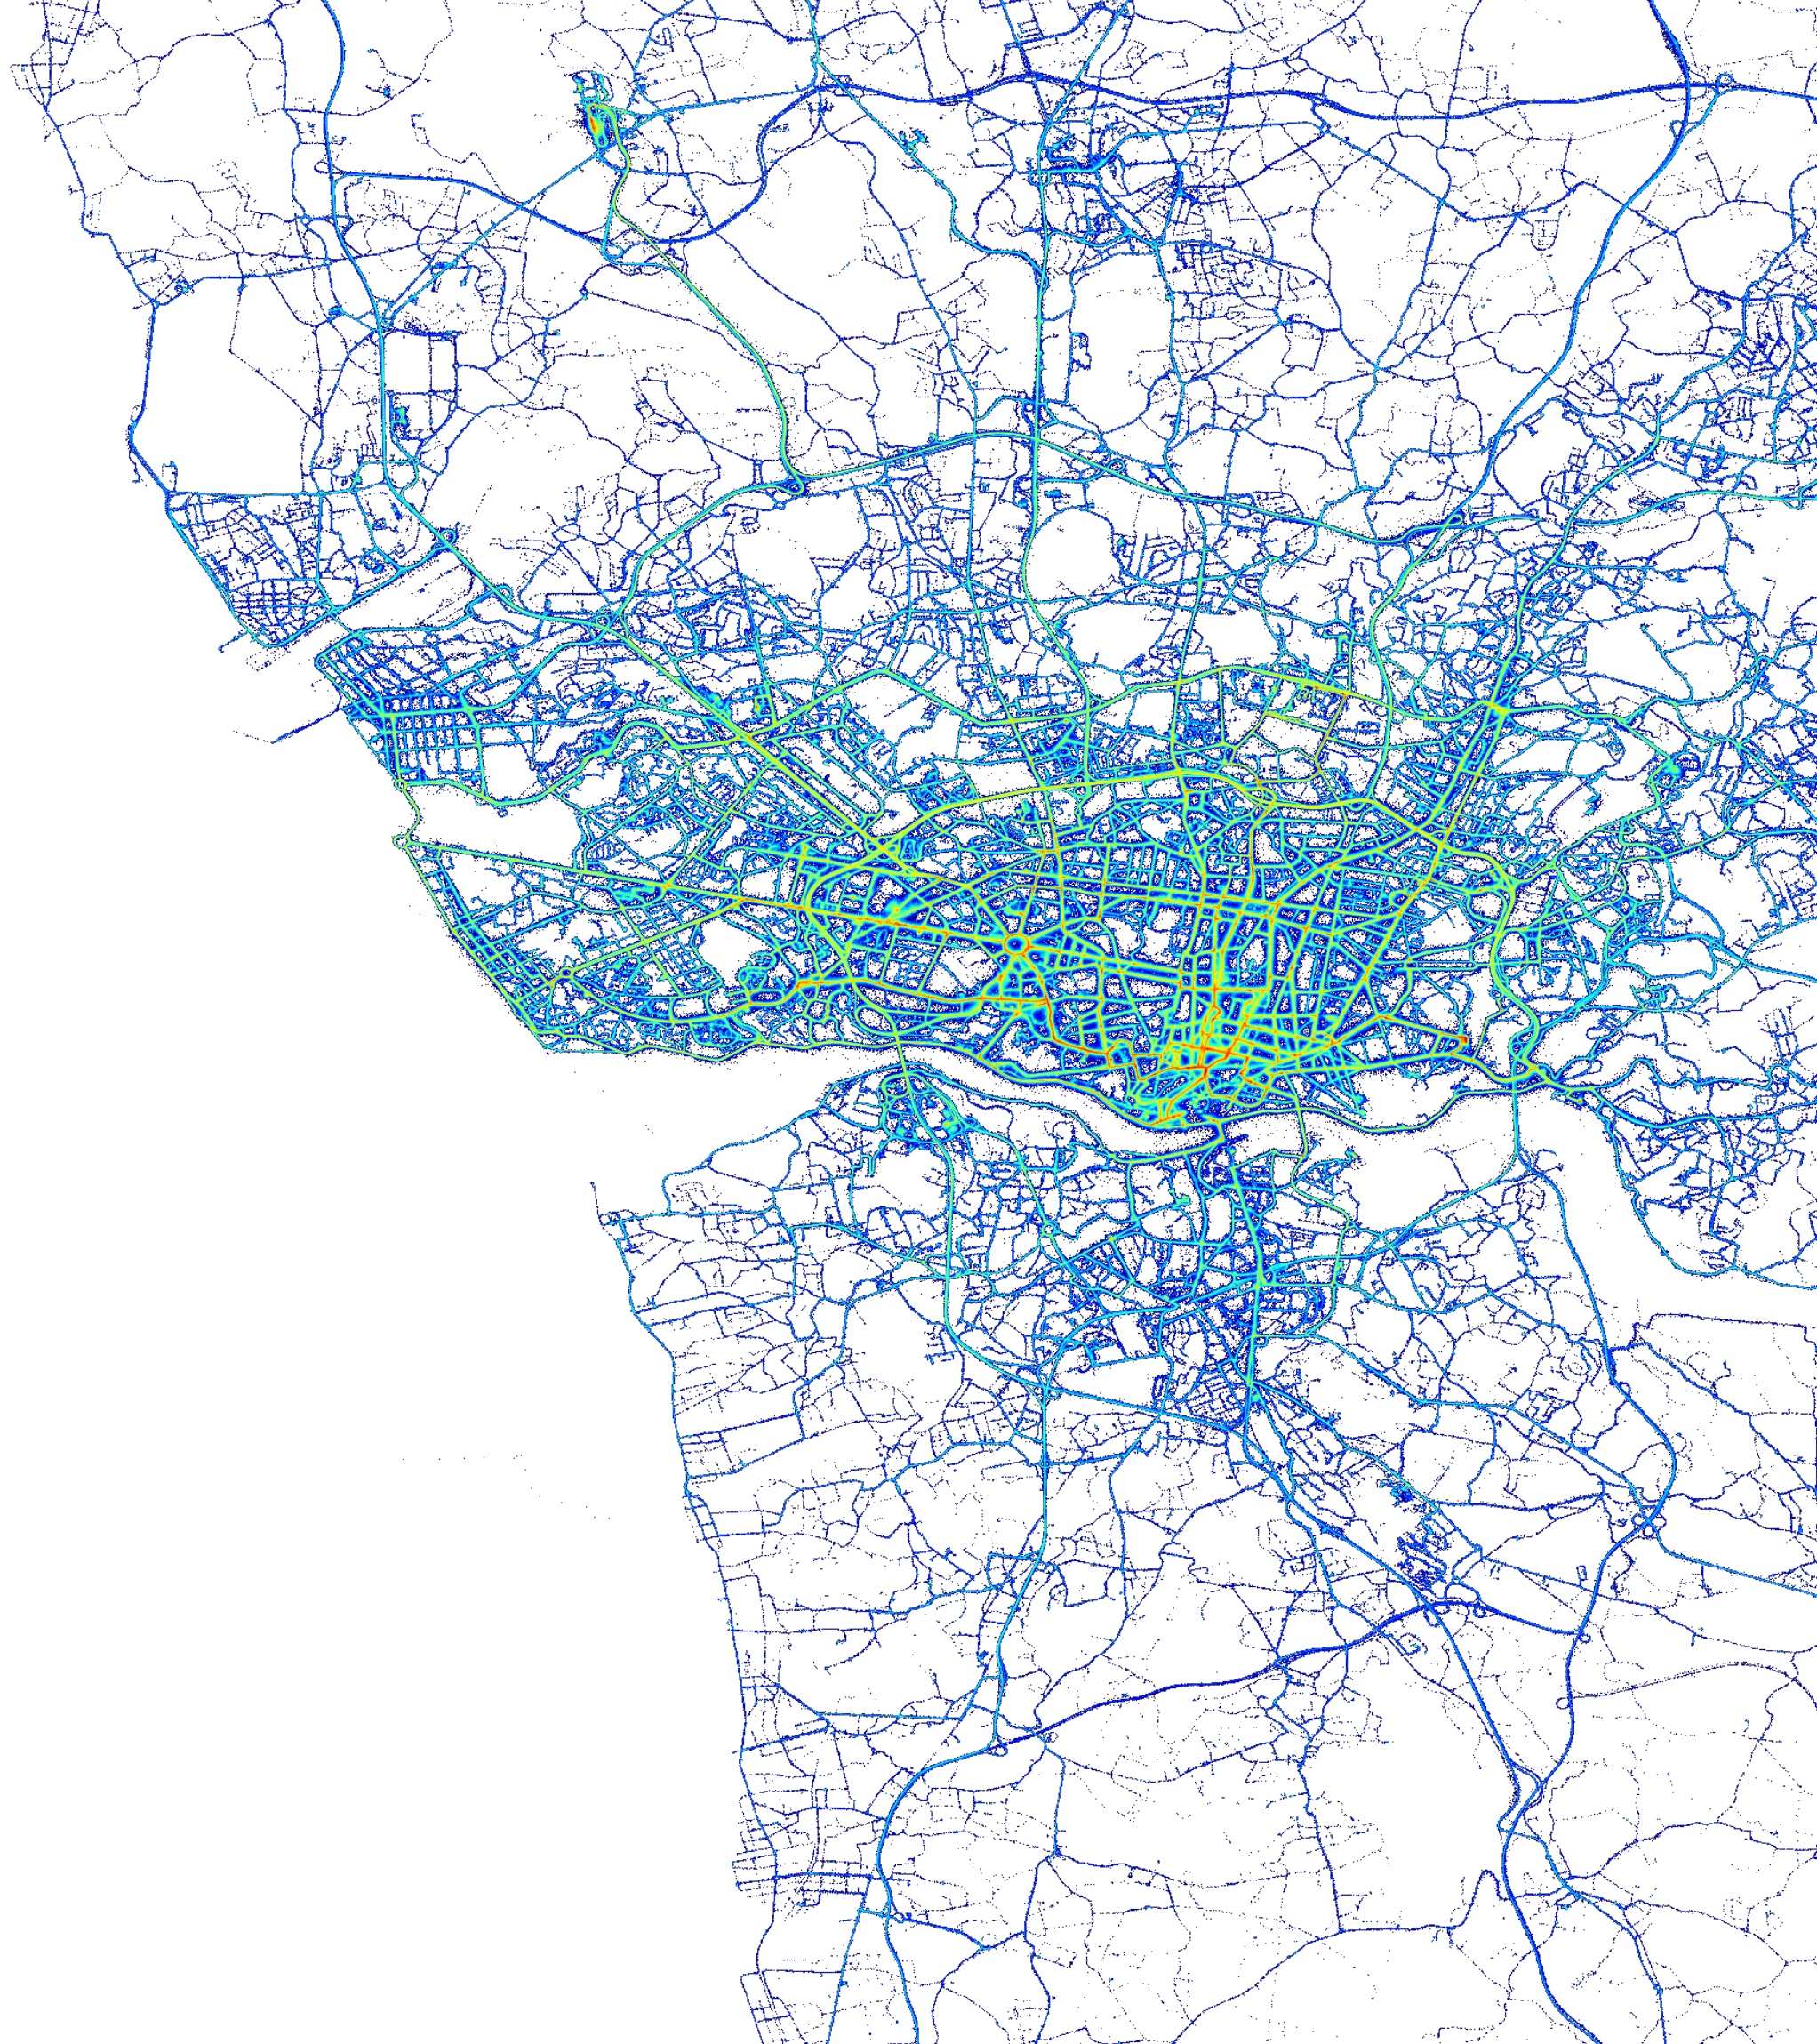
\includegraphics[height=0.85\textheight]{Figures/porto.png}
\end{frame}

\begin{frame}{Setup}
  \begin{itemize}
    \item 4-node cluster at DBLab.
    \item Processors: 8-core Intel(R) Xeon(R) CPU E3-1230 V2 @ 3.30GHz
    \item RAM: 15.5 GB.
    \item Centos 6.8, Simba/Spark 1.6.0.
  \end{itemize}
\end{frame}

\begin{frame}{Execution time}
  \centering
  \href{http://tinyurl.com/j9u9c7h}{\includegraphics[width=0.88\textwidth]{Figures/Porto_PBFE_N1M-16M_E2-10}}
\end{frame}

\begin{frame}{Scaleup}
  \centering
  \includegraphics[height=0.85\textheight]{Figures/Porto_Scaleup}
\end{frame}

\begin{frame}{Speedup}
  \centering
  \includegraphics[height=0.85\textheight]{Figures/Porto_Speedup}
\end{frame}

\section{Conclusions}

\begin{frame}{Conclusions}
  \begin{itemize}
   \item An implementation of a parallel method to detect disks for the BFE algorithm has been presented.
   \item The method proves to be scalable and reliable.
   \item Execution time improves up to 3 orders of magnitude compared to the sequential code.
  \end{itemize}

\end{frame}

\subsection*{Thanks...}

\begin{frame}{}
  \centering
  \huge Thank you!!! \\
  \vspace{2cm}
  \large Do you have any question?
\end{frame}

\end{document}